\draft Dirac cone of graphene.

\begin{parts}
	\part Close to the K point we have the Dirac cone as follows:
	\begin{figure}[H]
		\centering
		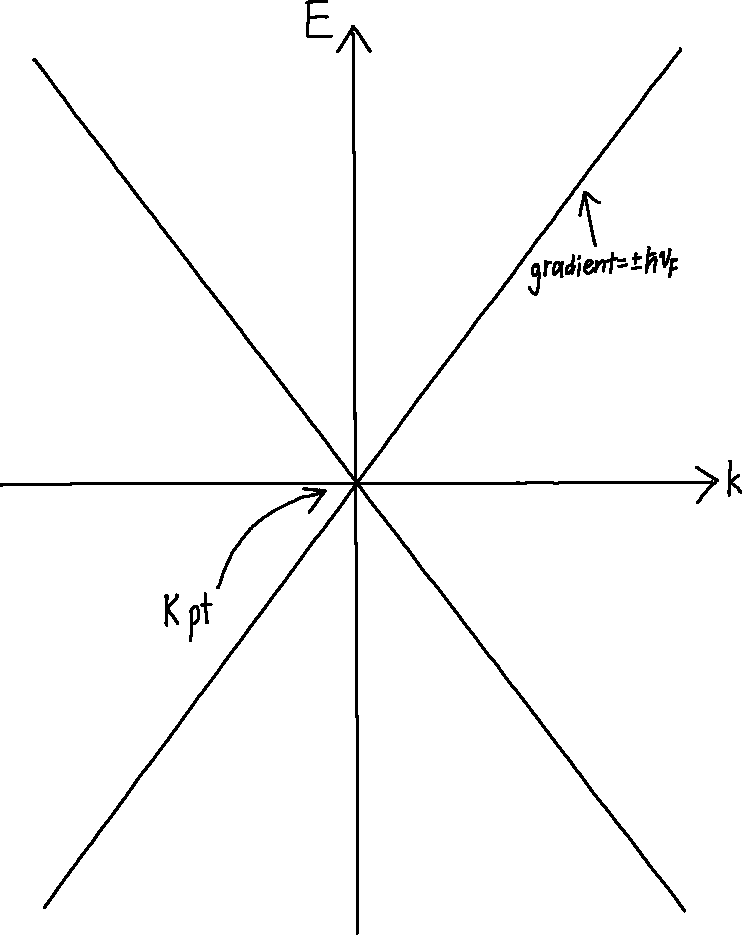
\includegraphics[width=.6\linewidth]{q6-dirac-cone}
	\end{figure}
	
	Resistance $R = V/I \propto E/J$ and $J = nqv \propto n$ so $R \propto 1/n$ the inverse of carrier density.
	Also note that around the K point, contour of constant energy is approximately a circle so the circumference determines the d.o.s. $\Rightarrow$ carrier density.
	Assuming $\mu = 0$ when the gate voltage is 0, we have the following sketch:
	\begin{figure}[H]
		\centering
		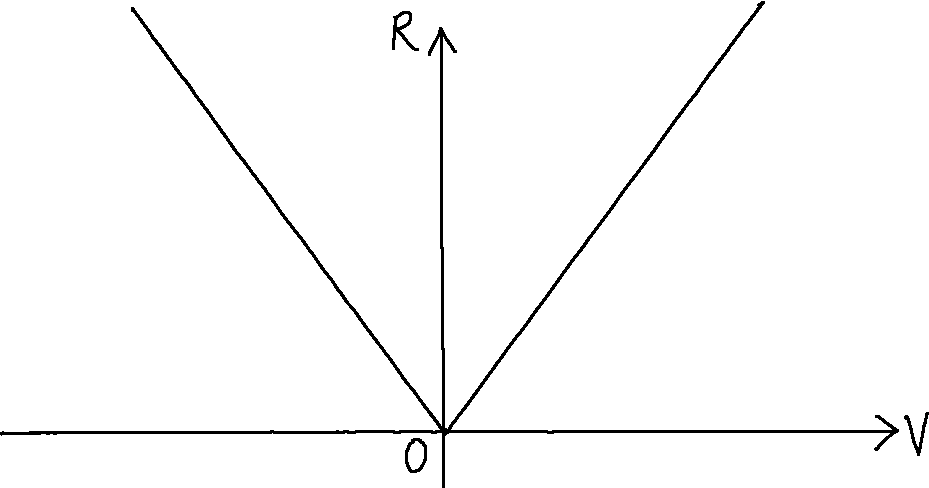
\includegraphics[width=.6\linewidth]{q6-rv}
	\end{figure}
	
	Landau levels have form:
	\begin{align*}
		E_l &= \rbracket{l + \frac{1}{2}} \hbar\omega_c \mtext{where $\omega_c = eB/m_{CR}$ is the cyclotron frequency} \\
		&= \frac{\hbar^2 k^2}{2m_{CR}} \\
		\Rightarrow k_l^2 &= \frac{2m_{CR}}{\hbar^2} \rbracket{l + \frac{1}{2}} \hbar \frac{eB}{m_{CR}} \\
		&\propto \frac{2eB}{\hbar}
	\end{align*}
	
	Hence $k_j$ has the form $\sqrt{\abs{2eB/\hbar}j}$.
	Plugging it into $E(k)$ then gives $E_j = v_\textnormal{F} \sqrt{\abs{2eB\hbar j}}$ as required.
	
	\# of states in a Landau level = $\Delta$(\# states between adjacent orbits)
	\begin{figure}[H]
		\centering
		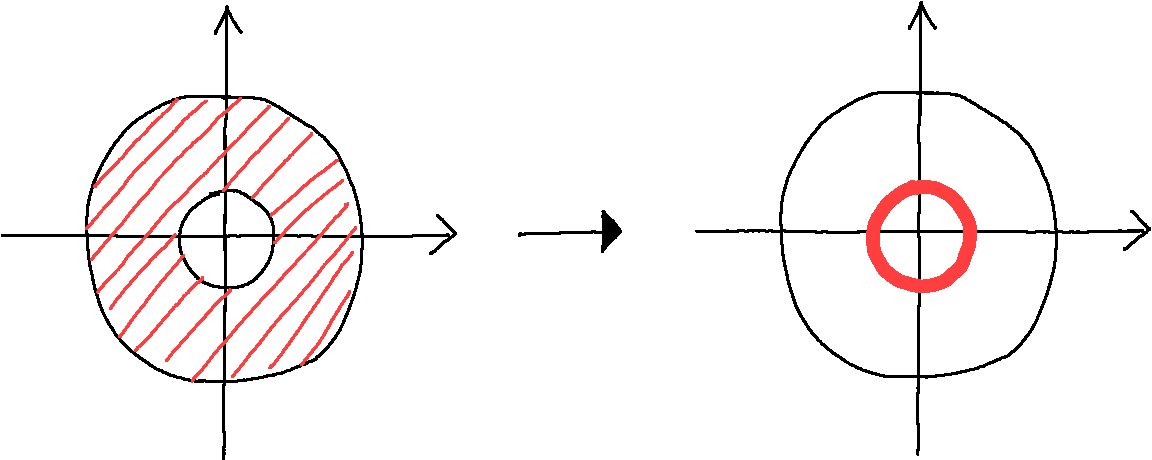
\includegraphics[width=.5\linewidth]{q6-landau-lvl}
	\end{figure}
	
	\begin{align*}
		N_j &= \underbracket{2}_{\textnormal{spin}} \cdot \underbracket{2}_{\textnormal{basis}} \cdot \frac{A}{\rbracket{2\pi}^2} \cdot \pi \underbracket{\rbracket{k_{j+1}^2 - k_j^2}}_{2eB/\hbar} \\
		\Rightarrow n_j &= \frac{2eB}{\pi\hbar} \mtext{in a Landau level}
	\end{align*}
	
	The areal density is then:
	\begin{align*}
		n &= n_j \cdot j \\
		&= \frac{2eB}{h/2} j \\
		&= \frac{4eB}{h} j
	\end{align*}
	
	Oscillatory period in $\Delta(1/B)$ for $n = \SI{1e16}{\per\metre\squared}$:
	\begin{align*}
		\Delta\rbracket{\frac{1}{B}} &= \frac{4e}{hn} \\
		&= \SI{0.097}{\per\tesla}
	\end{align*}
	
	When a Landau level is filled, there are no available holes for the electron to flow, hence $\rho_{xx} = 0$.
	At this stage, we are in the localised states where puddles of isolated conduction electrons are separated from one another, thereby making $\rho_{xy}$ constant.
	
	Sketch of $\rho_{xx}$ and $\rho_{xy}$ on the same axis:
	\begin{figure}[H]
		\centering
		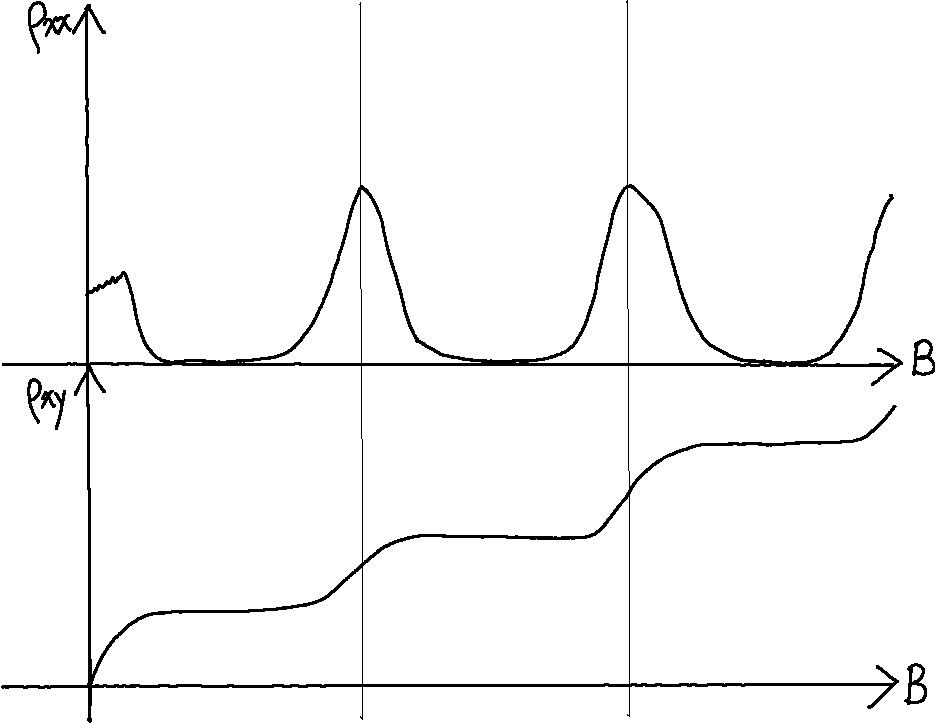
\includegraphics[width=.8\linewidth]{q6-rho}
	\end{figure}
	
	From Drude,
	\begin{align*}
		\deri{\mathbf{p}}{t} &= \mathbf{f} - \frac{\mathbf{p}}{\tau} \\
		\mathbf{p} &= \mathbf{f}\tau \mtext{at stationary state} \\
		m^* \mathbf{v} &= \rbracket{q \mathbf{v}\times\mathbf{B} + qE} \tau \\
		\frac{m^*}{nq} \hat{\mathbf{j}} &= q\tau \begin{vmatrix}
			\hat{\mathbf{x}} & \hat{\mathbf{y}} & \hat{\mathbf{z}} \\
			v_x & v_y & v_z \\
			B_x & B_y & B_z
		\end{vmatrix} + q\mathbf{E} \\
		&= q\tau \sbracket{v_y B_z \hat{\mathbf{x}} - v_x B_z \hat{\mathbf{y}}} + q\mathbf{E} \\
		&\Rightarrow \begin{cases}
			\frac{m^*}{nq} j_x = q\tau \cdot \frac{1}{nq} j_y B + qE_x \\
			\frac{m^*}{nq} j_y = -q\tau \cdot \frac{1}{nq} j_x B + qE_y \Rightarrow \frac{\tau}{nq} j_x B = E_y \mtext{since $j_y = 0$}
		\end{cases}
	\end{align*}
	
	Group velocity:
	\begin{align*}
		v_g &= \pderi{\omega}{k} \\
		&= v = \frac{1}{\hbar} \deri{E}{k}
	\end{align*}
	So we have $p = m^* v = \hbar k$:
	\begin{align*}
		\hbar k &= \frac{m^*}{\hbar} \deri{E}{k} \\
		\Rightarrow m^* &= \hbar^2 k \cdot \deri{k}{E} \\
		&= \frac{\hbar k}{v_\textnormal{F}}
	\end{align*}
	
	For quantum Hall effect to be well observed, we need:
	\begin{align*}
		\omega_c \tau = \frac{eB}{m^*}\tau = \frac{eBv_\textnormal{F}}{\hbar k}\tau &\gg 1 \\
		\Rightarrow eBv_\textnormal{F} \tau &\gg \hbar k \\
		\tau &\gg \frac{\hbar (\SI{1e9}{\per\metre})}{eBv_\textnormal{F}} = \SI{1.01e-13}{\second}
	\end{align*}
	
	Phonon broadening has the form:
	\begin{gather*}
		\hbar\underbracket{\omega_\textnormal{ph}}_{2\pi/\tau} \sim \boltzmann T \\
		\Rightarrow T_\textnormal{C} \simeq \frac{h}{\boltzmann \tau} = \SI{474}{\kelvin}
	\end{gather*}
\end{parts}